\section{Casi d'uso soddisfatti}
\subsection{Tabella del soddisfacimento dei casi d'uso}
\begin{table}[hp]
\centering
\begin{tabular}{|c|c|c|}
\hline
ID caso d'uso & Soddisfacimento nell'architettura & Soddisfacimento nel codice \\ \hline
UC1         & SODDISFATTO                       & NON SODDISFATTO                \\ \hline
UC2         & SODDISFATTO                       & NON SODDISFATTO                \\ \hline
UC3         & SODDISFATTO                       & NON SODDISFATTO                \\ \hline
UC4         & SODDISFATTO                       & NON SODDISFATTO                \\ \hline
UC6         & SODDISFATTO                       & SODDISFATTO                \\ \hline
UC7         & SODDISFATTO                       & SODDISFATTO                \\ \hline
UC8         & SODDISFATTO                       & SODDISFATTO                \\ \hline
UC9         & SODDISFATTO                       & SODDISFATTO                \\ \hline
UC10         & SODDISFATTO                       & SODDISFATTO                \\ \hline
UC11         & SODDISFATTO                       & NON SODDISFATTO                \\ \hline
UC12         & SODDISFATTO                       & NON SODDISFATTO                \\ \hline
UC13         & SODDISFATTO                       & NON SODDISFATTO                \\ \hline
UC14         & SODDISFATTO                       & NON SODDISFATTO                \\ \hline
UC15         & SODDISFATTO                       & NON SODDISFATTO                \\ \hline
UC16         & SODDISFATTO                       & NON SODDISFATTO                \\ \hline
UC17         & SODDISFATTO                       & NON SODDISFATTO                \\ \hline
UC18         & SODDISFATTO                       & NON SODDISFATTO                \\ \hline
UC19         & SODDISFATTO                       & NON SODDISFATTO                \\ \hline
UC20         & SODDISFATTO                       & NON SODDISFATTO                \\ \hline
UC21         & SODDISFATTO                       & NON SODDISFATTO                \\ \hline
UC22         & SODDISFATTO                       & NON SODDISFATTO                \\ \hline
UC23         & SODDISFATTO                       & SODDISFATTO                \\ \hline
UC24         & SODDISFATTO                       & NON SODDISFATTO                \\ \hline
UC25         & SODDISFATTO                       & NON SODDISFATTO                \\ \hline
UC26         & SODDISFATTO                       & NON SODDISFATTO                \\ \hline
UC27         & SODDISFATTO                       & SODDISFATTO                \\ \hline
UC28         & SODDISFATTO                       & SODDISFATTO                \\ \hline
UC29         & SODDISFATTO                       & NON SODDISFATTO                \\ \hline
UC30         & SODDISFATTO                       & SODDISFATTO                \\ \hline
UC31         & SODDISFATTO                       & SODDISFATTO                \\ \hline
UC32         & SODDISFATTO                       & SODDISFATTO                \\ \hline
UC33         & SODDISFATTO                       & SODDISFATTO                \\ \hline

\end{tabular}
\caption{Casi d'uso soddisfatti}
\end{table}
\clearpage

\subsection{Grafici sui casi d'uso soddisfatti}
\begin{figure}[hp]
\centering
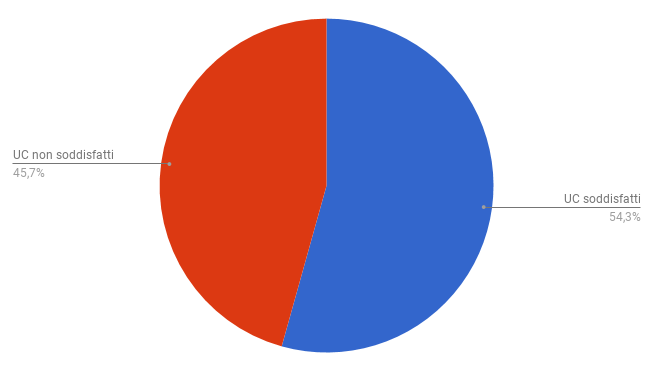
\includegraphics[height=7cm]{img/UCSoddisfatti.png}\\
\caption{Casi d'uso soddisfatti}
\end{figure}

